\documentclass{./assets/wfis}
\usepackage[utf8]{inputenc}
\usepackage{amsmath}
\usepackage{tabularx}
\usepackage[hidelinks]{hyperref}
\usepackage{afterpage}
\usepackage{biblatex} 
\addbibresource{assets/references.bib}

\usepackage{framed}
\usepackage{listings}
\usepackage[most]{tcolorbox}
\usepackage{hyphenat}
\usepackage{amsmath}
% \usepackage[inkscapeformat=png]{svg}
\usepackage[inkscapelatex=false]{svg}
\begin{document}

\tytul{Wykrywanie zmian stanu skupienia przy użyciu aparatu EEG}
\autor{Mateusz Kojro}
\nralbumu{389105}
\promotor{dr hab. Krzysztofa Wardy}
\katedra{Teorii Ciała Stałego}
\kierunek{informatyka}
\specjalnosc{informatyka stosowana}
\typpracy{inżynierska}
\specjalizacja{Algorytmy i Programowanie}


\stronatytulowa

\begin{abstract}

\end{abstract}

\chapter{Wstęp}

Układ nerwowy człowieka składa się z miliardów komórek nerwowych połączonych w gęstą siatkę pokrywającą całą powierzchnię ludzkiego ciała, w pełni kontrolując jego postrzeganie i interakcje z fizycznym światem odpowiada za rzeczy tak proste poruszanie pojedynczymi mięśniami przez dekodowanie rzeczywistości z nieskończonej kalkofoni impulsów dochodzących z wszystkich zmysłów az po kontrolowanie emocji tak skomplikowanych jak ciekawosc, zazdrośc czy miłość.

Na czele tego niezwykłego wynalazku ewolucji stoi mózg, nierozwiklana zagadka ktorej naukowcy i filozofowie poswiecali swoje zycia od czasow slawnego  . Dopiero niedawno opierając się na pracy niezliczonych osób pracujących w praktycznie wszystkich dziedzinach współczesnej nauki możliwe stało się rozkodowanie częsci tej niesamowitej tajemnicy. 

Praca przedstawia opracowanie oraz ewaluacje modelu klasyfikującego stan skupienia definiowany jako  xxxxx, za pomocą badania reakcji na bodziec z użyciem elektroencefalografii. 

W ramach projektu przygotowano układ eksperymentalny (sekcja \ref{aparatura-pomiarowa}), przeprowadzono kampanię badawczą na próbce xxxxx osób (sekcja \ref{procedura-badan}) której wyniki zostały następnie poddane analizie tradycyjnymi metodami statystycznymi (sekcja \ref{analiza-klasyczna}) uwzględniając zmienne zakłócające (sekcja \ref{zmiennne-zaklucajace}) oraz algorytmami uczenia maszynowego (sekcja \ref{uczenie-maszynowe}) kontrolując stronniczość (ang. bias) opracowanych modeli (sekcja \ref{bias}). Dyskusja wyników zaprezentowana została w rozdziale \ref{dyskusja}.

\section{Motywacja}
- Bo trwaja badania nad diagnozowaniem ADHD schizofremi itd, dodanie ML might be interesting

\section{Other Work}

Możliwość wykorzystania badania EEG w celu analizy stanu mentalnego pacjenta zaprezentowana została między innymi przez Kaushika i in. \cite{kaushik_decoding_2022} dodatkowo Guo i in. \cite{guo_detection_2018} pokazali, że możliwe jest klasyfikowanie stanu skupienia kierowcy w symulowanych warunkach. Wysoką skuteczność algorytmów uczenia maszynowego takich jak maszyny wektorów nośnych czy uczenie głębokie do analizy wyników elektroencefalografii udowodnili de Taillez i in. \cite{de_taillez_machine_2020}. 

Sprawnosc urzadzenia pomiarowego potwiedzili 

- Sekcja informujaca o rzeczach ktorych nie zrobili

\chapter{Podstawy teoretyczne}
\section{Model działania mózgu}
Pierwsze modele pracy mozgu stworzone zostaly juz w ... jednak dopiero

Ludzki mózg składa się z miliardów neuronów porozumiewających się między sobą za pomocą tzw. potencjałów czynnościowych – chwilowych impulsów, podczas których komórki znacząco zwiększają swoje wewnętrzne napięcie w celu przekazania sygnału do

Informacje w mózgu przekazywane i przetwarzane są za pomocą tzw. potencjałów czynnościowych – chwilowych impulsów, podczas których napięcie wewnątrz komórki stanowczo wzrasta (xxxx). Impuls taki zostaje wygenerowany gdy czasowo skalowana (xxxx) suma napiec na "wejściach" komórki (dendrytach) przekroczy pewien poziom (xxxx). W takiej sytuacji generowane jest napięcie, które następnie przekazywane jest za pomocą aksonu do kolejnych komórek (xxxxx)
\begin{equation}
    \text{Potencjał komórki} \approx 
    \begin{cases} 
      70mV & \sum_i d_i(t) > \text{Napięcie progowe}  \\
      -30mV &  \text{inaczej}
   \end{cases}
\end{equation}
gdzie $d_i(t)$ to napiecie na dendrycie $i$ w czasie $t$

- wspomniec huxley model
- Wspomniec ze it is all very variable
- Action potential happens when sum of time and strenght weighted inputs to the dendrites is higher than some treshold
- When the trigger level is achieved action potential is emited through the axon which is connected do dendrites of other cels - process continues
- bilions of those interactions form a working brain
- action potential is a high momentray increase in voltage in the neuron (i want the plot of the potential)

\section{Metody badania mózgu}


\begin{figure}[h]
    \centering
    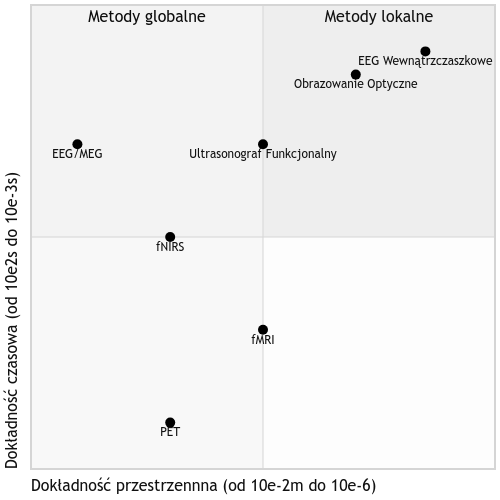
\includegraphics[width=0.5\columnwidth]{thesis/assets/porownanie_metod_badania_mozgu.png}
    \caption{Porównanie metod badania mózgu ze względu na dokładność czasową i przestrzenną}
    \label{fig:brain-imaging-comparasion}
\end{figure}


\section{EEG}
Elektroencefalografia (EEG) to badanie polegające na pomiarze potencjałów elektrycznych w różnych punktach na powierzchni głowy pacjenta. Zebrane w ten sposób informacje pozwalają na określenie względnej aktywności różnych obszarów mózgu.

Elektroencefalografia tradycyjnie wykorzystywana jest do diagnozowania schorzeń neurologicznych takich jak epilepsja, nowotwory mózgu czy zaburzenia snu. Podczas badania, operator wizualnie analizuje wykresy sygnałów o różnych częstotliwościach w czasie. W związku z relatywnie niskim poziomem sygnału do szumu oraz skomplikowanymi relacjami ukrytymi w wynikach oraz łatwy dostęp do aparatury pomiarowej pozwalający na stosunkowo proste zbieranie znaczących ilości danych rozpoczęto prace nad zastosowaniem algorytmów uczenia maszynowego w celu diagnozy innych jednostek chorobowych takich jak ADHD, dysleksja czy schizofrenia \cite{ahire_comprehensive_2022, joshi_review_2021, clarke_eeg_2002}.
\subsection{Mechanizm Działania}
% Potencjał czynnościowy (ang. \textit{action potential}) zmienia wewnętrzne napięcie neuronu o $\approx100mV$ na czas około $3ms$, biorąc pod uwagę odległość elektrod od źródła sygnału (natężenie pola elektrycznego spada z kwadratem odległości) oraz właściwości tłumiące tkanek ludzkich, pomiar aktywności pojedynczych neuronów za pomocą elektrod umieszczonych na skórze głowy jest niemożliwe.

Układ nerwowy człowieka przekazuje oraz przetwarza informacje za pomocą impulsów elektrycznych (potencjałów czynnościowych) wytwarzanych w komórkach nerwowych (neuronach), z pomocą mechanizmu xxxxx. Ze względu na dużą liczbę neuronów w ludzkim mózgu ($\approx10^9$\cite{herculano-houzel_human_2009}), ich małe rozmiary (xxxx) małe napięcie impulsu potencjału czynnościowego ($\approx100mV$\cite{biga_anatomy_2019}) oraz krótki czas jego trwania ($\approx2ms$\cite{biga_anatomy_2019}) niemożliwe jest badanie pracy pojedynczych neuronów, a jedynie średnich wartości milionów zsynchronizowanych impulsów na przestrzeni centymetrów (xxxxxx). Ograniczenia te powodują, że różne obszary mózgu mogą być badane z różną dokładnością (najlepszą sprawność otrzymuje się w rejonach mózgu znajdujących się blisko powierzchni skóry zawierających dużą liczbę tzw. neuronów piramidowych – np. kora przedczołowa).

\subsection{Metodyka Badania}

W zależności od specyfiki badania ważny jest dobór następujących parametrów:

\subsubsection{Rozmieszczenie oraz liczba elektrod}
Ogólnoprzyjętymi standardami pozycjonowania są tzw. międzynarodowe systemy $10$-$10$ i $10$-$20$ (przedstawiono na rysunku \ref{fig:10-20-system}), stosowanie tych metod pozwala na stosunkowo łatwe powielanie i porównywanie wyników badań przeprowadzonych w różnych placówkach. Alternatywnie 
% (nazewnictwo wywodzi się od procentowych podziałów czaszki – elektroda znajduje się co $10\%$ obwodu czaszki na osi przód – tył i co $20\%$ na osi prawo – lewo)

\begin{figure}[h]
    \centering
    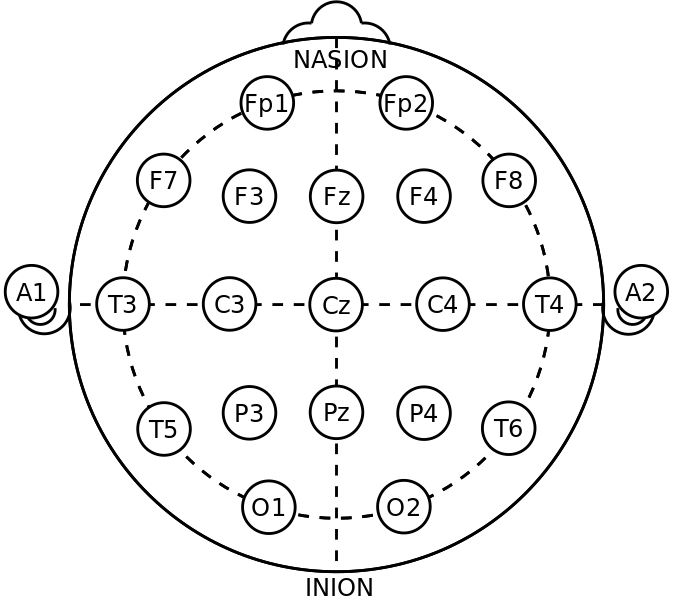
\includegraphics[width=0.5\columnwidth]{thesis/assets/10-20_system_electrodes.png}
    \caption{Rozmieszczenie elektrod w międzynarodowym systemie $10$-$20$}
    \label{fig:10-20-system}
\end{figure}

\subsubsection{Rodzaj elektrod}
Ze względu na jakość wyników, długość trwania badania oraz okoliczności towarzyszące badaniu konieczny jest dobór odpowiedniego typu elektrod. Najpopularniejsze z nich to:

\begin{itemize}
    \item \textbf{Elektrody żelowe} - Zapewniają wysoki poziom komfortu oraz dokładności pomiarów, wymagają aplikacji specjalnego żelu przewodzącego, utrudniając prowadzenie badań w warunkach terenowych.
    \item \textbf{Elektrody gąbkowe} - Pozwalają na kompromis pomiędzy jakością zebranych danych a łatwością aplikacji (żel przewodzący zamieniany jest na roztwór soli).
    \item \textbf{Elektrody suche} - Oferują najniższy poziom komfortu oraz dokładności, w zamian za bardzo wysoką łatwość użycia.
\end{itemize}

\subsubsection{Montaż}
Podczas badania EEG montażem nazywa się konfiguracje punktów odniesienia dla poszczególnych elektrod. Najbardziej popularnymi metodami montażu są:
% Some info in the summary of the book: https://docs.google.com/document/d/1bB9OZkO2m4fax8v3bGp_QZP7pAD-WryXQr4PxMppVp8/edit


\subsubsection{Badane częstotliwości}

\begin{table}[h]
    \centering
    \begin{tabular}{|c|c|c|}
        \hline
        Oznaczenie & Zakres częstotliwości & Zastosowanie \\
        \hline
        $\delta$ & $1$-$3Hz$ & \\
        $\theta$ & $4$-$7Hz$ & \\
        $\alpha$ & $8$-$12Hz$ & \\
        $\beta$  & $13$-$25Hz$ & \\
        $\gamma$ & $>25Hz$ & \\
        \hline
    \end{tabular}
    \caption{Typowe oznaczenia częstotliwości podczas badania EEG}
    \label{tab:freqs}
\end{table}
\chapter{Metody}

\section{Aparatura Pomiarowa}\label{aparatura-pomiarowa}

- w projekekcie napisalem ze to bedzie sterownik so i should make that clear

W celu przeprowadzenia badan aplikację webową pozwalającą na wyświetlanie bodźców na ekranie komputera (np. zadań matematycznych) oraz oprogramowanie serwerowe odpowiedzialne za sterowanie urządzeniem pomiarowym (Emotiv EPOCX), zbieranie informacji na temat odpowiedzi użytkownika, oraz korelowanie ich w czasie z mierzonym sygnałem EEG.

\subsection{Oprogramowanie}
- this should probably be pretty precise zeby nie bylo pytan czy to napewno jest praca inżynierska
- info o tym gdzie i jak zapisujemy wyniki
- info o konifguracji
 
Aplikacja stworzona na potrzeby badania składa się z 2 komponentów formularza zbierajacego infromacje na temat uczestnika oraz okoliczności, w jakich był on badany (\autoref{formularz-dla-osoby-badanej}) oraz modułu pozwalającego na wyświetlanie pytań w określonym interwale oraz zbieraniu na nie odpowiedzi. Na rysunku \ref{fig:app-flow} przedstawiono diagram typowego procesu działania aplikacji.

\begin{figure}[h!]
    \centering
    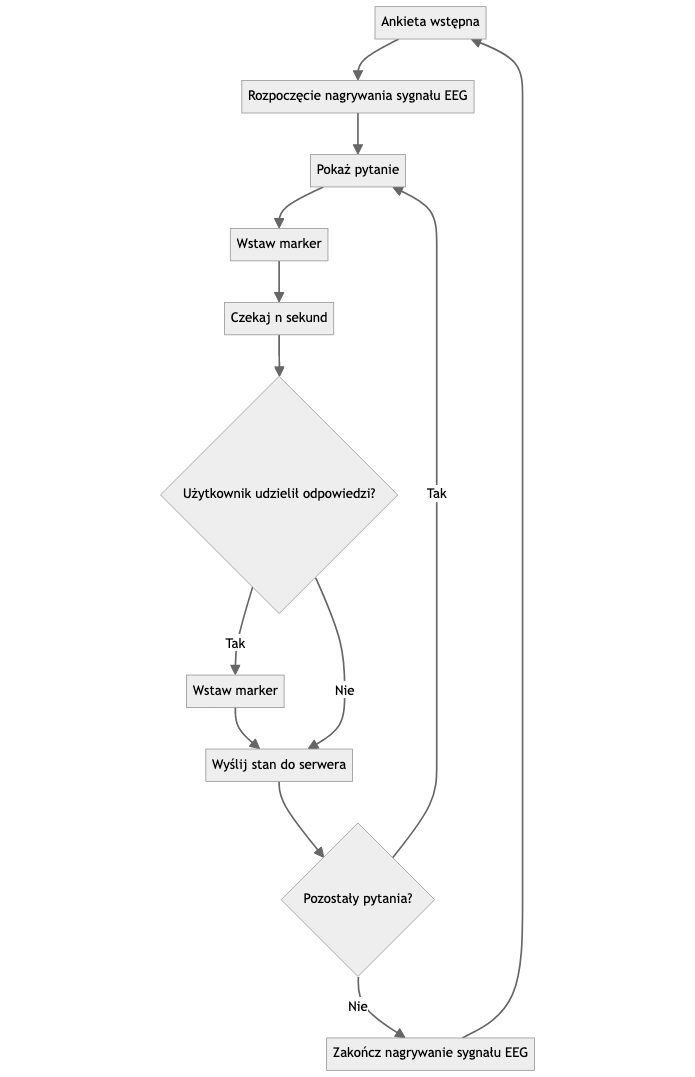
\includegraphics[width=0.5\columnwidth]{thesis/assets/app_flow_diagram.png}
    \caption{Typowy proces działania aplikacji}
    \label{fig:app-flow}
\end{figure}

Do wykonania oprogramowania wykorzystano

Oprogramowanie serwerowe jest niezależne od interfejsu graficznego aplikacji pozwalając na wykorzystanie przygotowanego REST API (dokumentacja znajduje się w załączniku \ref{api}) do implementacji innych eksperymentów wykorzystujących badanie EEG (w tym wykorzystanie wielu urządzeń jednocześnie).

Załącznik \ref{instrukcja} zawiera wymagania systemowe, opis pliku konfiguracyjnego oraz instrukcję instalacji i obsługi oprogramowania do zbierania danych.

\subsection{Urządzenie pomiarowe}\label{emotiv}
Do wykonania badan zdecydowano się na wykorzystanie 14 kanałowego (14 elektrod gąbkowych)  zestawu produkowanego przez firmę Emotiv (model EpocX). Wybór urządzenia podyktowany został dostępnością bibliotek pozwalających na interakcje z urządzeniem w czasie rzeczywistym (funkcjonalność wymagana w celu oznaczenia momentu wyświetlenia pytania oraz udzielenia na nie odpowiedzi) oraz obecnością wbudowanych czujników położenia i przyspieszenia (wymaganych w celu wyeliminowania zakłóceń związanych z ruchami głowy osoby badanej). Dodatkowo dołączone oprogramowanie pozwala na kalibrację przed, oraz monitorowanie w trakcie badania, jakości połączenia pomiędzy elektrodami a skórą pacjenta co pozwala na zmniejszenie ilości pomiarów zakończonych niepowodzeniem ze względów technicznych.

\section{Procedura przeprowadzonych badań}\label{procedura-badan}
- powtarzanie badan kiedy bylo to mozliwe
- przy powtórzeniach inny zestaw danych
\subsection{Ankieta wejściowa}
Przed przystąpieniem do badania ochotnikowi prezentowana jest ankieta wejściowa zawierająca informacje na temat badania (\autoref{opis-badania}), pytania na temat okoliczności badania i informacji demograficznych (\autoref{pytania-ankiety-wejsciowej}) oraz zgodę na przetwarzanie danych (\autoref{zgoda-na-przetwarzanie-danych}). Do momentu wyrażenia zgody, żadne informacje nie są zapisywane.

\subsection{Przygotowanie zestawu}
Przed przystąpieniem do badania gąbki znajdujące się na zakończeniach elektrod zamoczone zostały w roztworze soli fizjologicznej, następnie urządzenie umieszczone było na głowie badanej osoby a jakość połączenia sprawdzona za pomocą oprogramowania Emotiv Pro \cite{} jeżeli jakość przychodzących danych znajdowała się na zadowalającym poziomie (xxxx) pacjent proszony był o zamknięcie oczu na czas około 30 sekund w celu potwierdzenia poprawnej biokalibracji (przez weryfikację występowania wzrostu aktywności w zakresie częstotliwości $\alpha$).

\subsection{Badanie}
Po potwierdzeniu poprawnego działania urządzenia, w celu zapoznania ochotnika z działaniem interfejsu używanego do przeprowadzenia badania prezentowane są trzy przykładowe pytania. W razie braku pytań ze strony pacjenta operator opuszcza następnie pomieszczenie, a ochotnik rozpoczyna odpowiadać na pytania.

Badanie polega na serii zadań obliczeń arytmetycznych które ochotnik proszony jest o wykonanie bez wykorzystania żadnych narzędzi pomocniczych. Pytania zmieniane są automatyczne w konfigurowalnym interwale w tej samej kolejności dla każdego pacjenta, a udzielone odpowiedzi zapisywane jednocześnie sygnał EEG oraz informacje o przestrzenny położeniu urządzenia są nagrywane przez cały czas trwania badania, z markerami czasu wstawionymi w momentach wyświetlenia nowego pytania i udzielenia odpowiedzi na dane pytanie. W celu umożliwienia przeprowadzenia więcej niż jednego testu dla ochotnika przygotowano trzy różne zestawy pytań.


\section{Architektury algorytmów uczenia maszynowego}
- sieci neuronowe
    - rekurencyjne 
- random forest
- clustering algorithms
- svm

\chapter{Wyniki}
- publiczny dostep do zestawu dancyh
\section{Demografia}
- Wiek
- Płeć
- Wykształcenie
- Zawód
- Choroby neurologiczne/psychologiczne
- Stopien zaznajomienia z komputerami
\section{Zmienne zakłócające}\label{zmiennne-zaklucajace}
- Praca umsylowa danego dnia
- Poziom zmeczenia
- Otoczenie (miejscie zamieszkania obce znajome)
- Pora dnia
- Godziny snu poprzedniej nocy
- Uzywki (kawa, papierosy) w ciagu ostatnich 6h
\section{Standard analysys}\label{analiza-klasyczna}
\subsection{ANOVA}
\subsection{Fourier}
- odseparowac momenty wyswietlenia pytania i udzielenia odpowiedzi i porownac z stanem domyslnym
- porownac czestotliwosci na poczatku badania i na koncu
- interesujace korelacje z innymi zmiennymi (maybe macierz korelacji)
\section{Uczenie maszynowe}\label{uczenie-maszynowe}
- confusion matrices
\section{Bias analysys - Shaply values}\label{bias}
- wiek
- plec

\chapter{Dyskusja}\label{dyskusja}

\appendix
\chapter{Formularze dla osób badanych}\label{formularz-dla-osoby-badanej}
\section{Opis badania}\label{opis-badania}
\section{Zgoda na przetwarzanie danych}\label{zgoda-na-przetwarzanie-danych}
\section{Pytania ankiety wejściowej}\label{pytania-ankiety-wejsciowej}
\section{Pytania zawarte w badaniu}\label{pytania-badania}
\chapter{Instrukcja uruchomienia i obsługi oprogramowania}\label{instrukcja}
\section{Wymagania systemowe}
\section{Instalacja}
\section{Obsługa}
\section{Konfiguracja}
\chapter{Dokumentacja API}\label{api}
- register questions endpoint
- register answer
- mark point

\printbibliography

\clearpage
\listoffigures
\clearpage
\listoftables
\clearpage

\end{document}